\documentclass[11pt, a4wide]{mwart}

\usepackage{polski}
\usepackage{a4wide}
\usepackage[utf8]{inputenc}
\usepackage{hyperref}

\usepackage{amssymb}
\usepackage{amsmath}
\usepackage{amsthm}
\usepackage{algorithmicx}
\usepackage{algorithm}
\usepackage{graphicx}
\usepackage{epstopdf}
\usepackage{algpseudocode}
\usepackage{float}

\newtheorem{definition}{Definicja}


\title{Algorytm ewolucyjny dla problemu superstringu}
\author{Jan Sochiera \and Krzysztof Chrobak}

\begin{document}
\maketitle
\tableofcontents



\section{Problem}
Problem superstringu polega na znalezieniu najkrótszego słowa $W$, którego
podsłowami są słowa z danego zbioru $S = \{w_1, w_2, ..., w_n\}$ nad alfabetem
$\Sigma$. Zadanie to jest NP-zupełne \cite{GJ}, ale wymyślono dla niego kilka
wielomianowych algorytmów o różnych współczynnikach aproksymacji. W naszym
projekcie próbowaliśmy rozwiązać ten problem przy pomocy algorytmu ewolucyjnego
i prostej heurystyki.

\begin{definition}[problem superstringu] 
Mając dany zbiór słów $S = \{w_1, w_2, ..., w_n\}$ znaleźć najkrótsze słowo
$W$, które zawiera wszystkie słowa z $S$ jako spójne podciągi.  
\end{definition}

Problem ten można nieco uprościć, wymagając by $S$ był \emph{factor-free}.

\begin{definition}[factor-free] 
Zbiór słów $S$ jest factor-free, jeśli dla dowolnych $u, v \in S$ $u$ nie jest
podsłowem $v$.  
\end{definition}

Oczywiście z dowolnego zbioru słów $S$ można zrobić zbiór $S'$ o tej własności,
i rozwiązanie problemu superstringu dla $S'$ jest też rozwiązaniem dla $S$. W
dalszej części tekstu pisząc "zbiór słów" będziemy mieli na myśli zbiór
factor-free.


\subsection{Przestrzeń poszukiwań}
Jeśli przez $b_1, b_2 ... b_n$ oznaczymy pozycje na których zaczynają się i
kończą $w_1, w_2 ..., w_n$ w ich superstringu $W$, to zauważymy że kolejność
tych pozycji definiuje pewną permutację elementów zbioru $S$.

\begin{definition}[nałożenie] 
$ov : \Sigma^* \times \Sigma^* \rightarrow \mathbb{N}$, dla słów $u, v \in \Sigma^*$ 
$ov(u, v) = k$ wtedy i tylko wtedy gdy $k$ to największa liczba spełniająca:
\begin{itemize}
  \item $k \leq min(|u|, |v|)$
  \item $u[(|u| - k + 1) ... |u|] = v[1...k]$
\end{itemize}
Czyli mówiąc po polsku jest to najdłuższy sufiks $u$, który jest jednocześnie prefiksem
$v$.
\end{definition}


\begin{definition}[sklejenie]
Sklejeniem słów $u$ i $v$ będziemy nazywali słowo $w = u[1...|u|]v[ov(u, v) ... |v|]$.
Operację tą oznaczymy jako $w = glue(u, v)$.
\end{definition}

Oczywiście przestrzenią poszukiwań jest $S_n$, ponieważ sklejając $w_1 ... w_n$ w kolejności
rosnących $b_i$ dostaniemy superstring $W$. 

\subsection{Funkcja celu}
Definiujemy funkcję celu $f : S_n \rightarrow \mathbb{N}$ jako długość superstringu otrzymanego
przez wykonanie poniższego algorytmu:

\begin{algorithm}[H]
\caption{Definicja funkcji celu}
\label{funkcja celu}
\begin{algorithmic}
  \Function{f}{$\pi$}
    \State $super \gets \epsilon$
    \For{$i = 1 ... n$}
    \State $super \gets glue(super, w_{\pi[i]})$
    \EndFor
    \State \Return $|super|$
  \EndFunction
\end{algorithmic}
\end{algorithm}




\section{Algorytm ewolucyjny}
Algorytm zastosowany do tego problemu w dużej części pochodzi z naszego 
poprzedniego projektu \cite{flowshop}, więc przedstawimy jego ogólny zarys
i dokładnie opiszemy różnice, nie zagłębiając się w szczegóły części wspólnej.
Pseudokod algorytmu znajduje się na listingu~\ref{algorytm}.

\begin{algorithm}[H]
\caption{Algorytm ewolucyjny dla problemu flow shop}
\label{algorytm}
\begin{algorithmic}
  \State $instance \gets Preprocess(instance)$
  \State $P \gets RandomPopulation(population\_size)$
  \State $EvaluatePopulation(P, instance)$
  \While{not $TerminationCondition(P)$}
    \State $Parents \gets SelectParents(P, num\_parents)$ 
    \State $Children \gets Crossover(Parents)$
    \State $Children \gets Mutate(Children, mutation\_probability)$
    \State $Children \gets LocalSearch(Children, instance)$
    \State $Population \gets Replace(Population, Children)$
    \State $Population \gets AddImigrants(Population, instance, \alpha)$
  \EndWhile
\end{algorithmic}
\end{algorithm}



\subsection{Preprocessing $Preprocess$}
W tej fazie algorytmu dla każdej pary słów $u, v$ z instancji problemu 
przy pomocy algorytmu KMP \cite{jewels} sprawdzamy, czy $u$ nie zawiera się w
$v$, i zapamiętujemy wartość $ov(u, v)$. Algorytm KMP pozwala nam wykonać obie
te czynności w czasie $O(max(|u|, |v|))$, więc cały preprocessing ma złożoność
$O(n ^ 2 * maxlen)$, gdzie $maxlen$ to najdłuższe słowo w instancji problemu.

Eksperymentowaliśmy z zastosowaniem drzew sufiksowych, ale niestety stała
ukryta w teoretycznie lepszej złożoności algorytmu Ukkonena \cite{ukkonen} i
potrzebna pamięć spowodowały, że zastosowaliśmy prostsze podejście do tego
problemu.

\begin{algorithm}[H]
\caption{Preprocessing}
\label{preprocessing}
\begin{algorithmic}
  \Function{Preprocess}{instance}
  \State $OV \gets new\ Array[n, n]$
  \For{$i = 1...n$}
    \For{$j = 1.. n$}
      \If{$i \neq j \land KMP\_Find(instance[i], instance[j]$}
        \State $instance.remove\_later(j)$
      \EndIf
      \State $OV[i, j] = ov(instance[i], instance[j])$
    \EndFor
  \EndFor
  \EndFunction
\end{algorithmic}
\end{algorithm}


\subsection{Ocena osobników $EvaluatePopulation$}
Aby ocenić pojedynczego osobnika, wystarczy od sumy długości słów w problemie
odjąć sumę wartości $ov$ par jego kolejnych elementów. Formalnie:

$$ f(\pi) = \sum\limits_{i = 1}^n |w_i| - \sum\limits_{i = 1}^{n - 1} ov(w_{\pi[i]}, w_{\pi[i + 1]})$$


\subsection{Operator krzyżowania $Crossover$}
By wykorzystać wiedzę o problemie, zastosowaliśmy zmodyfikowany operator OX, w
którym jako punkty rozerwania rodzica wybieramy miejsca, gdzie nałożenie dwóch
kolejnych słów jest najmniejsze.


\subsection{Przeszukiwanie lokalne $LocalSearch$}
Przeszukiwanie lokalne dla danego osobnika polega na przejrzeniu wszystkich
permutacji, które można z niego uzyskać przez jedną transpozycję. Takie
podejście umożliwia ocenienie każdego z $\frac{n(n-1)}{2}$ sąsiadów w czasie $O(1)$.
Poniżej pokażemy przekształcenia dla osobnika $\pi$ w którym zamieniamy
miejscami słowa $1 < i < i+1 < j < n$, żeby nie rozpraszać się przypadkami
szczególnymi. $\pi' = \pi \cdot (i, j)$


\begin{eqnarray*}
f(\pi') &=& \sum\limits_{t = 1}^n |w_t| - \sum\limits_{t = 1}^{n - 1} ov(w_{\pi'[t]}, w_{\pi'[t + 1]}) \\
        &=& \sum\limits_{t= 1}^n |w_t| -
          \sum\limits_{t = 1 \atop t \not \in \{i-1, i, j-1, j\}}^{n - 1} ov(w_{\pi'[t]}, w_{\pi'[t + 1]}) \\
          & & + ov(w_{\pi'[i-1]}, w_{\pi'[i]}) + ov(w_{\pi'[i]}, w_{\pi'[i+1]}) \\
          && + ov(w_{\pi'[j-1]}, w_{\pi'[j]}) + ov(w_{\pi'[j]}, w_{\pi'[j+1]}) \\
        &=& \sum\limits_{t = 1}^n |w_i| -
          \sum\limits_{t = 1 \atop t \not \in \{i-1, i, j-1, j\}}^{n - 1} ov(w_{\pi'[t]}, w_{\pi'[t + 1]}) \\
          && + ov(w_{\pi[i-1]}, w_{\pi[j]}) + ov(w_{\pi[j]}, w_{\pi[i+1]}) \\
          && + ov(w_{\pi[j-1]}, w_{\pi[i]}) + ov(w_{\pi[i]}, w_{\pi[j+1]}) \\
        &=& f(\pi) \\
          && + ov(w_{\pi[i-1]}, w_{\pi[j]}) + ov(w_{\pi[j]}, w_{\pi[i+1]}) \\
          && + ov(w_{\pi[j-1]}, w_{\pi[i]}) + ov(w_{\pi[i]}, w_{\pi[j+1]}) \\
          && - ov(w_{\pi[i-1]}, w_{\pi[i]}) - ov(w_{\pi[j]}, w_{\pi[j+1]}) \\
          && - ov(w_{\pi[j-1]}, w_{\pi[j]}) - ov(w_{\pi[j]}, w_{\pi[j+1]}) 
\end{eqnarray*}




\newpage
\section{Algorytm heurystyczny}
Prosta heurystyka z którą się porównujemy działa zgodnie z poniższym schematem \ref{heurystyczny}:

\begin{algorithm}[H]
\caption{Algorytm heurystyczny}
\label{heurystyczny}
\begin{algorithmic}
\State$L \gets []$
\For{$i = 1...n$}
  \For{$j = 1.. n$}
    \State $append(L, (OV[i, j], i, j))$
  \EndFor
\EndFor
\State $Sort(L)$
\State $super \gets \sum\limits_{t = 1}^n |w_t|$
\While{$size(L) \neq 0$}
  \State $(k, i, j) \gets L.back()$
  \State $L.pop\_back()$
  \If{koniec $w_i$ oraz początek $w_j$ nie są z niczym połączone}
    \If{$w_i$ oraz $w_j$ nie należą do jednego segmentu superstringu}
      \State $super \gets super - k$
      \State oznacz koniec $w_i$ jako połączony
      \State oznacz koniec $w_j$ jako połączony
      \State zapamiętaj że $w_i$ oraz $w_j$ są w jednym segmencie superstringu
    \EndIf
  \EndIf
\EndWhile

\end{algorithmic}
\end{algorithm}

Algorytm zachłannie łączy słowa o największym dostępnym pokryciu, a na koniec jego działania
w zmiennej $super$ znajduje się długość superstringu

Nie jest to algorytm aproksymacyjny, ponieważ nie pokazano dotąd dolnego ograniczenia na jakość
zwracanego rozwiązania, ale nie znaleziono do tej pory przypadku, dla którego dawałby rozwiązanie
dwukrotnie gorsze niż optymalne.





\section{Implementacja}
Implementacja algorytmu w dużej części bazuje na programie z naszego poprzedniego projektu, 
w którym zmieniliśmy przeszukiwanie lokalne, ocenianie osobnika i operator krzyżowania.

\subsection{Kompilacja}
Potrzebne programy:
\begin{itemize}
  \item Kompilator obsługujący OpenMP, np. GCC 4.7
  \item CMake
\end{itemize}
Polecenia do skompilowania załączonego programu:
\begin{enumerate}
  \item \verb|tar -xvf superstring.tar|
  \item \verb|cd superstring/program|
  \item \verb|mkdir build|
  \item \verb|cd build|
  \item \verb|cmake .. -DCMAKE_BUILD_TYPE=Release|
  \item \verb|make|
\end{enumerate}
Jeśli kompilacja przebiegnie pomyślnie, wygenerowane zostaną programy:
\begin{description}
  \item[genetic] implementacja algorytmu ewolucyjnego
  \item[random] implementacja losowego przeszukiwania przestrzeni permutacji
  \item[heuristic] implemetacja algorytmu heurystycznego
\end{description}
Każdy z nich uruchomiony bez żadnych opcji wyświetli krótką instrukcję obsługi.






\section{Wyniki eksperymentów}

\subsection{Przejrzenie całej przestrzeni poszukiwań}
Aby dowiedzieć się, jak dla małych wartości $n$ wygląda rozkład funkcji celu w
całej przestrzeni poszukiwań, postanowiliśmy wyliczyć jej wartość dla całego
$S_n$.  Wykres \ref{rozklad_liniowo} przedstawia "dystrybuantę" (tj. \%
permutacji o wartości funkcji $f$ mniejszej bądź równej danej) $f$ w $S_{11}$
na skali liniowej. Na wykresie \ref{rozklad_logarytmicznie} znajduje się
początkowy fragment tego wykresu na skali liniowej. Wykresy te sugerują, że
praktycznie niemożliwe jest znalezienie optymalnego rozwiązania przez
zgadywanie, natomiast aż 50\% populacji jest nie gorsza niż półtora optimum,
więc nie będzie trudno znaleźć "akceptowalne" rozwiązanie.

\begin{definition}[współczynnik jakości]
Współczynnik jakości $Q$ osobnika $\pi$ to iloraz 
$ Q(\pi) = \frac{f(\pi)}{f(\pi_{opt})}$
gdzie $\pi_{opt}$ to optymalne rozwiązanie.
\end{definition}

\begin{figure}[H]
\caption{Liniowy wykres dystrybuanty rozkładu $f$ w $S_{11}$}
\label{rozklad_liniowo}
\begin{center}
  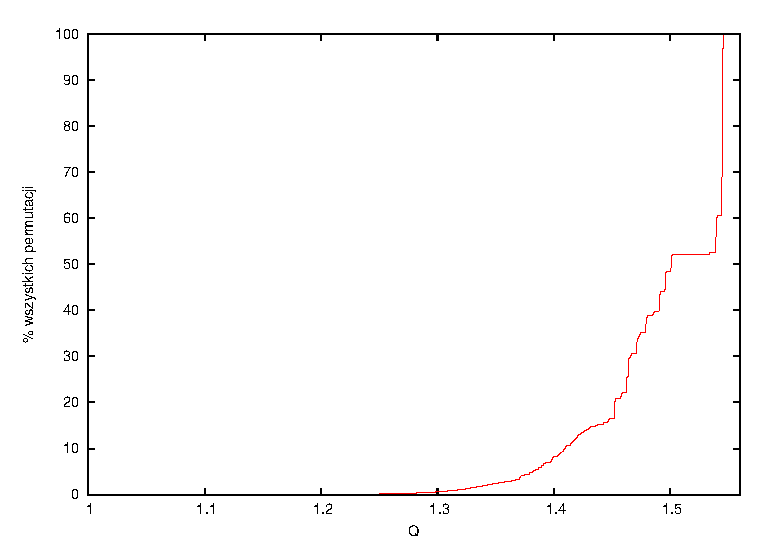
\includegraphics{dystrybuanta_bez_logarytmicznej.eps}
\end{center}
\end{figure}


\begin{figure}[H]
\caption{Logarytmiczny wykres dystrybuanty rozkładu $f$ w $S_{11}$}
\label{rozklad_logarytmicznie}
\begin{center}
  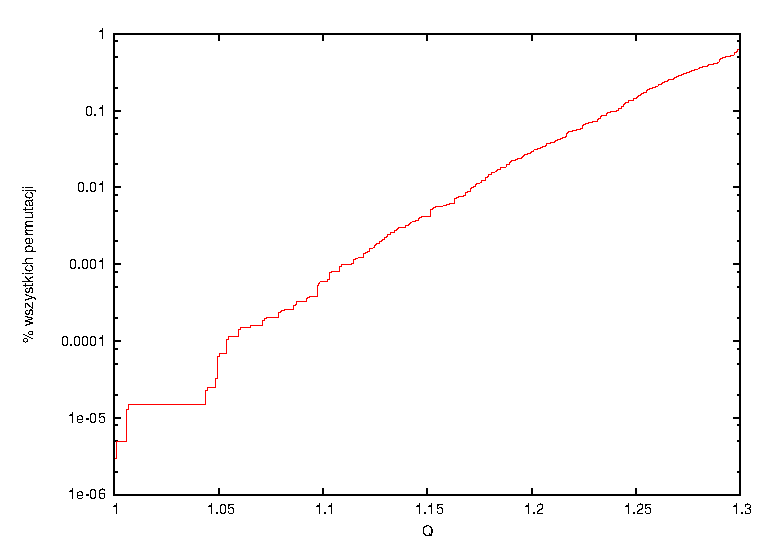
\includegraphics{dystrybuanta_logarytmiczna.eps}
\end{center}
\end{figure}



\subsection{Benchmarki}
Ze względu na trudność w znalezieniu benchmarków postanowiliśmy
wygenerować je na własną rękę.  Funkcja generująca przykładowy problem
do rozwiązania pobiera 3 argumenty: oczekiwaną długość superstringu,
liczbę słów które ma utworzyć oraz procentowy overlap. Benchmark
generowany jest zgodnie z algorytmem \ref{generator}.


\begin{algorithm}[H]
\caption{Generowanie benchmarków}
\label{generator}
\begin{algorithmic}
  
  \State utwórz superstring o zadanej długości
  \State podziel superstring na zadaną liczbę słów o tej samej długości
  \State każde ze słów rozszerz o podany współczynnik zmodyfikowany losowo
  w taki sposób, aby dalej pozostawało podsłowem
  \State losowo pozamieniaj kolejność otrzymanych słów

\end{algorithmic}
\end{algorithm}



Dla uproszczenia testowania algorytmów w wygenerowanych zestawach
testowych wybraliśmy długość stringu równą $50000$ oraz procentowy
overlap równy $70\%$ dla każdego zestawu.  Mieliśmy nadzieję, że takie
współczynniki wystarczą do tego, by oczekiwana długość superstringu
mogła w każdym zestawie testowym posłużyć za wartość optymalną. Ale
algorytmy potrafiły znaleźć jeszcze lepsze wartości. Dzieje się tak ze
względu na niewielki rozmiar alfabetu, jakiego użyliśmy.  Jednakże
znajdowane rozwiązania nigdy nie były znacznie lepsze od oczekiwanego,
a ponieważ nigdy nie możemy mieć pewności, że zadana długość
superstringu będzie optymalnym  rozwiązaniem, nawet dla bardzo dużego
alfabetu i overlapów, zdecydowaliśmy się użyć wygenerowanych
benchmarków i posługiwać się wartością $50000$ jako orientacyjną.





\subsection{Jakość rozwiązań}
W celu oceny naszych rozwiązań zaimplementowaliśmy dwa dodatkowe algorytmy
rozwiązujące problem superstringu: random i heurystyczny. Działanie algorytmu
heurystycznego zostało już opisane, a działanie algorytmu "random" zgadza się z
jego nazwą, ponieważ polega na wylosowaniu i ocenieniu pewnej liczby osobników.

Nasze eksperymenty polegały na dwudziestokrotnym uruchomieniu algorytmu
ewolucyjnego i losowego na tych samych danych, oraz jednokrotnym użyciu
algorytmu heurystycznego (ponieważ jest deterministyczny). 

Ze względu na specyfikę algorytmu oceniania funkcji celu, "random" nie był w
stanie ocenić tylu osobników co ewolucyjny w rozsądnym czasie, więc
przerywaliśmy jego pracę po czasie równym czasowi pracy ewolucyjnego. 

Tabela \ref{parametry} przedstawia wartości parametrów algorytmu ewolucyjnego 
dla których uzyskaliśmy przedstawione niżej wyniki.

\begin{table}[H]
\caption{Wartości parametrów algorytmu}
\label{parametry}
\begin{center}
\begin{tabular}{l|c}
  \hline
  parametr & wartość \\
  \hline
  rozmiar populacji & 2000 \\
  ilość rodziców & 2000 \\
  prawdopodobieństwo mutacji & 0.05 \\
  $\alpha$ & 0.3 \\
  \hline
\end{tabular}
\end{center}
\end{table}


\begin{table}[H]
\caption{Najlepsze znalezione rozwiązanie}
\label{best}
\begin{center}
\begin{tabular}{c|c|c|c}
  \hline
  $n$ & ewolucyjny & random & heurystyka\\
  \hline
  100 & 49985 & 80775 & 49318 \\
  200 & 50000 & 82697 & 49543 \\
  400 & 57209 & 83779 & 49823\\
  600 & 58640 & 84110 & 49764 \\
  800 & 63133 & 83178 & 49571 \\
  1000 & 65681 & 83297 & 49938 
\end{tabular}
\end{center}
\end{table}



\begin{table}[H]
\caption{Średnie rozwiązanie}
\label{mean}
\begin{center}
\begin{tabular}{c|c|c}
  \hline
  $n$ & ewolucyjny & random\\
  \hline
  100 & 49985 & 80775 \\
  200 & 50194 & 82768 \\
  400 & 57893 & 83779 \\
  600 & 58732 & 84120 \\
  800 & 63152 & 83183 \\
  1000 & 65858 & 83301
\end{tabular}
\end{center}
\end{table}



\begin{table}[H]
\caption{Odchylenie standardowe znajdowanych rozwiązań}
\label{sdev}
\begin{center}
\begin{tabular}{c|c|c}
  \hline
  $n$ & ewolucyjny & random\\
  \hline
  100 & 0 & 0 \\
  200 & 258 & 40.7 \\
  400 & 530 & 0 \\
  600 & 176 & 15.8 \\
  800 & 42 & 10 \\
  1000 & 94 & 6.5
\end{tabular}
\end{center}
\end{table}



\subsection{Przebieg obliczeń}
Przebieg obliczeń wykonywanych przez algorytm ewolucyjny postanowiliśmy zobrazować
przy pomocy trzech wskaźników - wartości funkcji celu dla najlepszego osobnika
w populacji, średniej wartości funkcji celu w populacji i wartości współczynnika 
różnorodności $D$. Wykresy \ref{wykres_600} oraz \ref{diversity_600} pokazują te
wartość w funkcji numeru iteracji.


\begin{definition}[współczynnik różnorodności] 
Współczynnikiem różnorodności $D$ populacji $P$ nazwiemy wartość ilorazu
$D = \frac{\text{ilość różnych osobników}}{|P|}$
\end{definition}



\begin{figure}[H]
\caption{Przebieg obliczeń dla $n = 600$ }
\label{wykres_600}
\begin{center}
  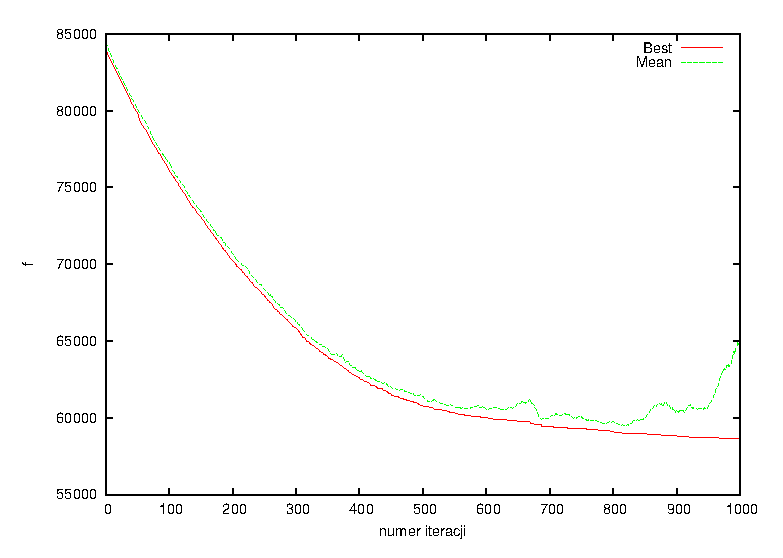
\includegraphics{wykres_600.eps}
\end{center}
\end{figure}


\begin{figure}[H]
\caption{Wartości $D$ dla $n = 600$ }
\label{diversity_600}
\begin{center}
  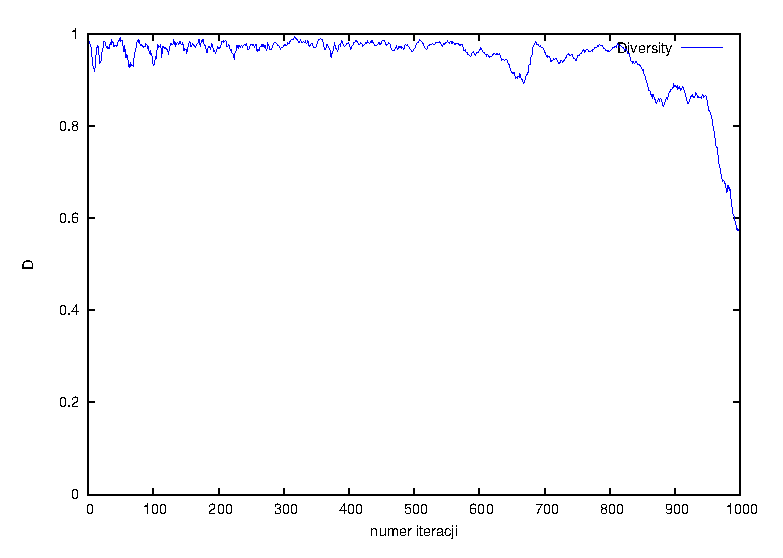
\includegraphics{wykres_diversity_600.eps}
\end{center}
\end{figure}



\subsection{Czas działania}
Złożoność algorytmu jest zdominowana przez przeszukiwanie lokalne, które dla
pojedynczego osobnika trwa aż $O(n^2)$. Jeśli ilość osobników w populacji
oznaczymy przez $k$, ilość iteracji przez $s$ a długość najdłuższego słowa z $S$
przez $maxlen$, to teoretyczna złożoność algorytmu wyniesie:

$$ O(\underbrace{n^2 \cdot maxlen}_{\text{preprocessing}} + 
  \underbrace{n^2 \cdot k \cdot s}_{\text{właściwe obliczenia}}) $$

W tabeli \ref{czas} znajduje się średni czas wykonania jednej iteracji
algorytmu dla różnych wartości $n$, wygenerowanych przez nas benchmarków i
wartościach parametrów z tabeli \ref{parametry}.  Testy przeprowadziliśmy na
komputerze z 4GB pamięci RAM i procesorem Intel i5 $4\times2.5$ GHz. Algorytm
heurystyczny radził sobie z problemem znacząco szybciej, ponieważ
dla największego testu $n = 1000$ jego czas działania wyniósł 0.5s.

\begin{table}[H]
\caption{Średni czas jednej iteracji algorytmu}
\label{czas}
\begin{center}
\begin{tabular}{c|c}
  \hline
  $n$ & czas \\
  \hline
  400 & 3s \\
  500 & 5s \\
  600 & 9s \\
  700 & 15s \\
  800 & 23s \\
  900 & 30s \\
  1000 & 36s \\
\end{tabular}
\end{center}
\end{table}





\subsection{Zużycie pamięci}
Poza pamięcią potrzebną na przechowanie problemu, program potrzebuje $O(n \cdot
k)$ ($k$ - ilość osobników) komórek pamięci na populację, i $O(n^2)$ komórek na
przechowanie informacji uzyskanych podczas preprocessingu. Nie mierzyliśmy
dokładnie ile wyniosło zapotrzebowanie dla poszczególnych problemów, ponieważ
asymptotyczne oszacowanie sugerowało że nie będzie to czynnik ograniczający
rozmiar problemu rozwiązywalnego naszym algorytmem.




\section{Wnioski}

\subsection{Nasz algorytm a algorytm losowy}
Dane z tabel \ref{best} i \ref{mean} pokazują, że nasz algorytm nie sprowadza
się tylko do losowego błądzenia po przestrzeni poszukiwań, ponieważ osiąga
znacznie lepsze wyniki niż random. Ciekawe jest porównanie wyników z tabeli
\ref{sdev}, które pokazują odchylenie standardowe wszystkich 20 eksperymentów
dla każdej instancji problemu. O ile nasz algorytm zgodnie z oczekiwaniami
osiąga różne wyniki, to random zachowuje się interesująco, dla wielu testów
dając dwudziestokrotnie podobne wyniki.  Takie nieoczekiwane zachowanie tego
algorytmu jest prawdopodobnie wynikiem rozkładu wartości funkcji celu w
przestrzeni rozwiązań, gdzie łatwo jest trafić na osobnika o średniej jakości,
natomiast bardzo trudno na osobnika znacząco lepszego niż większość możliwych.


\subsection{Nasz algorytm a heurystyka}
Heurystyka jest lepsza od naszego algorytmu ewolucyjnego pod każdym względem.
Jej czas działania (dla największego testu 0.5s) i jakość osiąganych rozwiązań
powodują, że to właśnie jej używa się do rozwiązywania tego problemu w praktyce.


\subsection{Działanie naszego algorytmu}
Dzięki losowej imigracji i ostrożnej selekcji, różnorodność populacji pozostaje 
na wysokim poziomie nawet po wielu iteracjach, co pokazuje wykres \ref{diversity_600}.
Umożliwia to niemal dowolnie długie obliczenia, podczas których nie dojdzie do zastąpienia
całej populacji kopiami jednego osobnika. Wpływ imigracji widać szczególnie gdy zestawi się
wykresy \ref{wykres_600} i \ref{diversity_600}, bo w momencie spadku różnorodności 
dodanie wielu losowych osobników do populacji powoduje spadek średniej wartości
funkcji celu.







\begin{thebibliography}{}
\bibitem{GJ} 
Michael Garey, David S. Johnson
"Computers and Intractability: A Guide to the Theory of NP-Completeness"

\bibitem{flowshop}
Jan Sochiera, Krzysztof Chrobak
"Algorytm ewolucyjny dla problemu flow shop"

\bibitem{jewels}
Crochemore, Maxime; Rytter, Wojciech "Jewels of Stringology"

\bibitem{ukkonen}
E. Ukkonen. (1995). "On-line construction of suffix trees"

\end{thebibliography}





\end{document}


